\section{Ladder Operator Block-Encoding (LOBE)}
\label{sec:lobe}

In this section of the text, we'll do the following:
\subsection{Defining "Block-Encoding"}
\label{subsec:block-encoding}

\subsection{Prior Works}
\label{subsec:prior-works}

\subsubsection{Linear Combination of Unitaries}

\subsubsection{Sparse Block-Encoding of Pairing Hamiltonians}
stuff from Liu et al
\ws{Might ask you to fill this out @Gus}

\subsection{Rescaling of Coefficients Due to Bosonic Terms}
\label{subsec:rescaling}


\subsection{Circuit Construction}
\label{subsec:circuit}

\begin{figure}
    \centering
    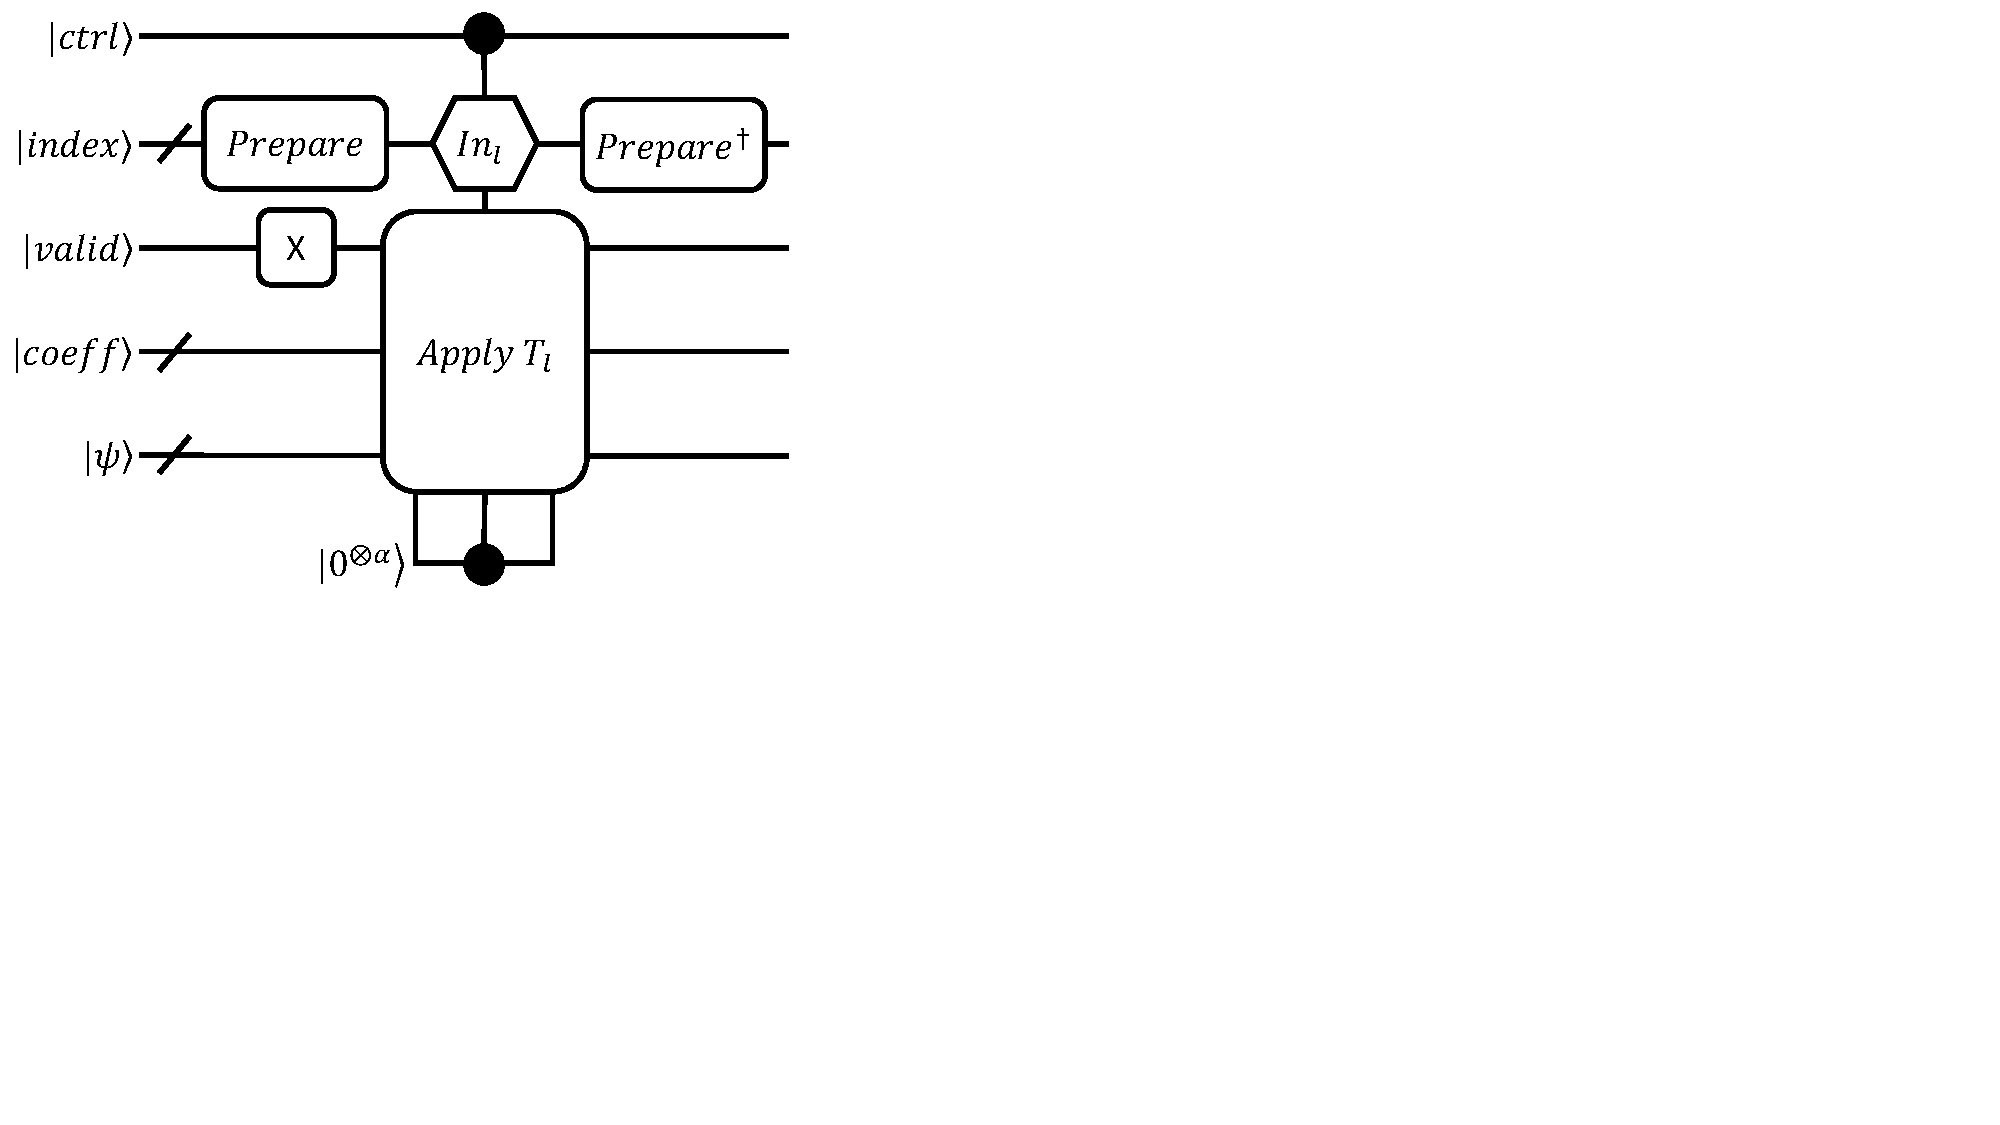
\includegraphics[width=8cm]{figures/lobe-block-encoding.pdf}
    \caption{\textbf{Ladder Operator Block-Encoding.}
    }
    \label{fig:lobe}
\end{figure}

In Figure \ref{fig:lobe}, we define the LOBE circuit in terms of generic oracles.
Disregarding the (optional) control qubit ($\ket{\textit{ctrl}}$), the LOBE circuit makes use of 5 qubit registers: $\ket{\textit{index}}$, $\ket{\textit{valid}}$, $\ket{\textit{coeff}}$, $\ket{\psi}$, and $\ket{0^{\otimes \alpha}}$.

The register denoted $\ket{\textit{index}}$ is referred to as the index register and is used to index the terms in the Hamiltonian as is done in LCU constructions. 
The integer representations of the computational basis states of the index register corresponds to the indices $l$ in Eq. \ref{eq:lclo}. 

The register denoted $\ket{\textit{valid}}$ consists of a single qubit and is referred to as the validation qubit.
It serves the same purpose as in \cite{liu2024efficient} which is to denote whether or not the term at the current index ($T_l$) will annihilate the quantum state.
If the term will annihilate the state, then the validation qubit remains in the $\ket{1}$ state such that the branch of the wavefunction stays outside the desired subspace of the block-encoding.
If the term will not annihilate the state, then the validation qubit gets flipped to the $\ket{0}$ state for the term $T_l$.

The register denoted $\ket{\textit{coeff}}$ is referred to as the coefficient register and is used to apply the coefficients associate with the term $T_l$. 
These coefficients include both the coefficients of the terms in the linear combination ($\alpha_l$) as well as the coefficients associated with the bosonic ladder operators.
One qubit is used to apply the $\alpha_l$ coefficient while a separate qubit will be required for each bosonic operator (defined as a creation, annihilation, or occupation operator acting with a positive integer-valued exponent) in the term.

The register denoted $\ket{\psi}$ is referred to as the system register and is used to encode the state of the system.
This register can be broken up into three subsequent registers: the fermionic system $\ket{\psi_b}$, the antifermionic system ($\ket{\psi_d}$), and the bosonic system ($\ket{\psi_a}$).
The encoding studied in this work is outlined in more detail in Subsection \ref{subsec:encoding}.

Finally, the register denoted $\ket{0^{\otimes \alpha}}$ is referred to as the clean ancillae register.
This register includes ancillae qubits that are promised to begin in the $\ket{0}$ state and are returned to this state at the end of the block-encoding circuit.

The LOBE circuit is structured similarly to an LCU circuit in that it involves sequential application of a $\textit{Prepare}$ oracle, a $\textit{Select}$ oracle, and then uncomputing the $\textit{Prepare}$ oracle using the daggered circuit.
In addition to these oracles, a single $X$ gate is applied to the $\ket{\textit{valid}}$ qubit in order to prepare this qubit in the $\ket{1}$ state.
This single $X$ gate is \textit{not} repeated on subsequent applications of the block-encoding.

\subsubsection{Prepare Oracle}
The $\textit{Prepare}$ oracle is applied to the index register to prepare a superposition over the computational basis states of this register.

\textbf{Uniform State Preparation}

The simplest implementation of the $\textit{Prepare}$ oracle is to prepare a uniform superposition over the computational basis states using a series of Hadamard gates on each qubit in the register.
The rescaling condition for this implementation is that the coefficients must be rescaled such that they all have magnitude $\leq 1$.
Let the largest coefficient magnitude be given by $\alpha^* = \max{|\alpha_l|}$.
Then, this rescaling imposes a constant rescaling factor on the Hamiltonian of $1 / \alpha^*$
We refer to these rescaled coeffifients as $\Tilde{\alpha_l}$.
An additional rescaling factor of $2^{-\lceil \log_2{L} \rceil}$ from the uniform superposition results in an overall rescaling of the Hamiltonian by a constant factor of:
\begin{equation}
    \lambda_{usp} = \frac{1}{2^{\lceil \log_2{L} \rceil} \alpha^*}
\end{equation}

The quantum resource requirements of this implementation of $\textit{Prepare}$ are negligible as no ancillae are required and only Clifford operations (Hadamards) are performed.
However, this implementation of $\textit{Prepare}$ requires that the rescaled coefficients of the terms ($\Tilde{\alpha_l}$) be incorporated within the $\textit{Select}$ oracle which will be described in Subsubsection \ref{subsubsec:select}.

\textbf{Arbitrary State Preparation}

An alternative implementation of $\textit{Prepare}$ is to use the same implementation traditionally used in LCU circuits.
The coefficients are first rescaled by their $L1-norm$:
\begin{equation}
    \lambda_{asp} = \sum_{l=0}^{L-1} |\alpha_l|
\end{equation}
Then, a state preparation routine is applied that performs the following operation:
\begin{equation}
    \ket{0^{\otimes \lceil \log_2{L} \rceil}} \rightarrow_{\textit{Prepare}} \sum_{l = 0}^{L-1} \sqrt{|\alpha_l| / \lambda} \ket{l}
\end{equation}
This results in a weighted superposition over the computational basis states where the squared amplitudes of the basis states are equal to the magnitude of the associated coefficients.

For Hamiltonians that have structure among the coefficients of the terms, implementations of the $\textit{Prepare}$ oracle can be constructed that leverage this structure.
In certain cases, this can drastically reduce the cost of $\textit{Prepare}$ such as is done for the Fermi-Hubbard model in \cite{babbush2018encoding}.
However, when a certain structure cannot be assumed, the Grover-Rudolph algorithm from \cite{grover2002creating} gives a formulaic routine to generate these $\textit{Prepare}$ circuits.

Gover-Rudolph requires $L-1$ rotations, with $1$ being uncontrolled and the others controlled.
The implementation also requires several series of multiplexing.
\ws{I think we can make the implementation use fewer Toffolis by doing some smart multiplexing.}
The total number of Toffolis \ws{(if my assumption is correct)} is given by:
\begin{equation}
    N_{\textit{toff}} = \lfloor \frac{L}{2} \rfloor
\end{equation}
and the total number of ancillae is given by:
\begin{equation}
    Q_{asp} = \lceil \log_2{L} \rceil - 2
\end{equation}
\ws{check this.}
It should be noted that these ancillae, which will be returned to $\ket{0}$ after the oracle call completes, will likely be reused in the $\textit{Select}$ oracle and therefore will not contribute to the total qubit requirement of the block-encoding.

\subsubsection{Select Oracle}
\label{subsubsec:select}

\begin{figure}
    \centering
    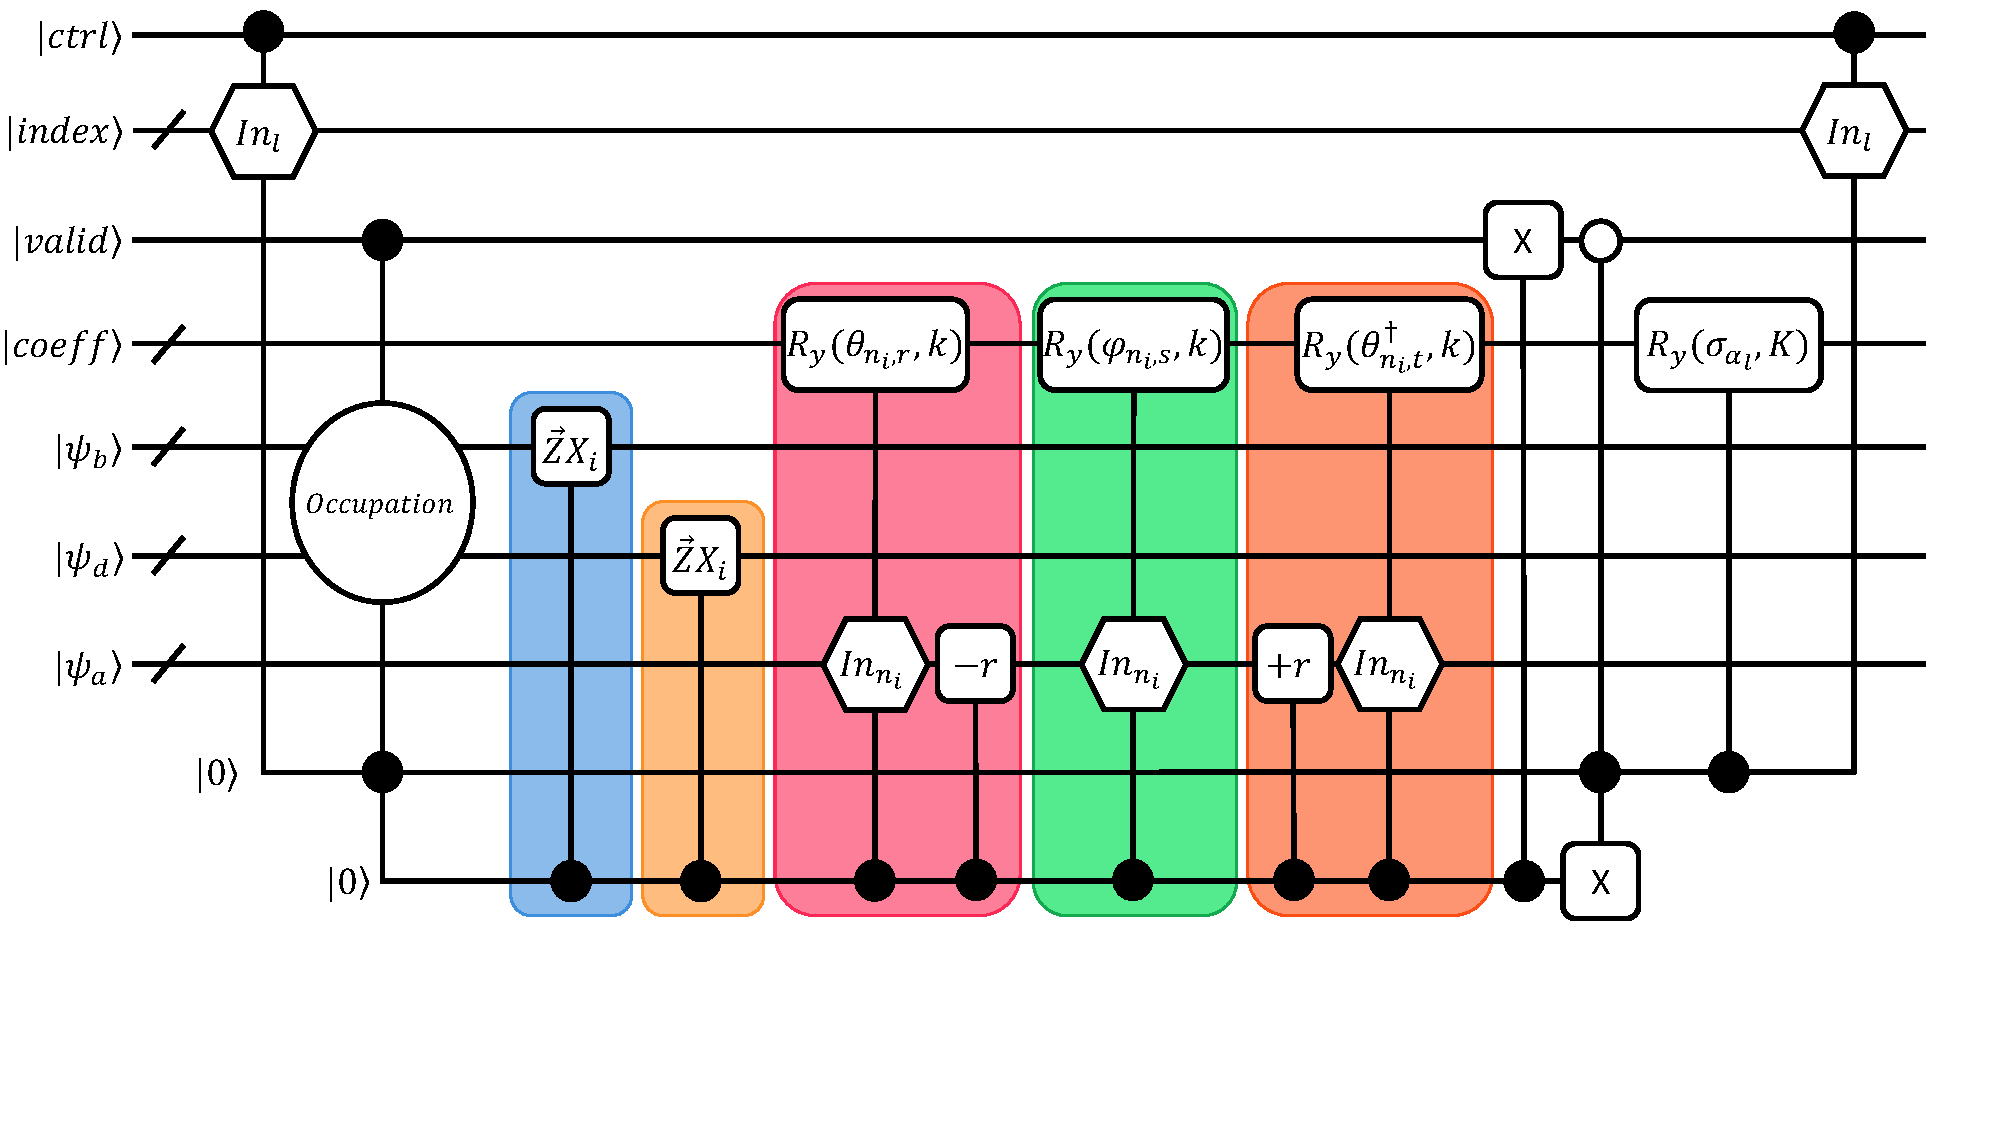
\includegraphics[width=16cm]{figures/applying-term.pdf}
    \caption{\textbf{Ladder Operator Term Oracle.}
    }
    \label{fig:lobe-term}
\end{figure}


\subsection{Analytical Cost Analysis}
\label{subsec:analytics}

The minimum number of qubits required for the index register is given by:
\begin{equation}
    Q_{\textit{index}} = \lceil \log_2{L} \rceil
\end{equation}

If we let $K$ denote the maximum number of bosonic operators within a single term, then the minimum number of qubits in the coefficient register is given by:
\begin{equation}
    Q_{\textit{coeff}} = K + 1
\end{equation} 

Using the qubit-efficient encoding described in Subsection \ref{subsec:encoding}, the minimum number of qubits required for the system registers is given by:
\begin{equation}
    \begin{split}
        &Q_{\psi_b} = \Lambda \\
        &Q_{\psi_d} = \Lambda \\
        &Q_{\psi_a} = \Lambda \lceil \log_2{(\Omega + 1)} \rceil
    \end{split}
\end{equation} 

There are numerous space-time tradeoffs that one can make to either reduce the number of ancillae qubits at the cost of more gates or vice versa.
In this work, we opt for compilations that minimize the number of non-Clifford operations at the expense of more ancillae qubits.
With this choice, the number of clean ancillae required is given by:
\begin{equation}
    \alpha = \lceil \log_2{L} \rceil + (B + 1) + \lceil \log_2{(\Omega + 1)} \rceil
\end{equation}
where $\lceil \log_2{L} \rceil$ qubits are used for multiplexing over the index register, $ \lceil \log_2{(\Omega + 1)} \rceil$ qubits are used for multiplexing over the bosonic occupation registers, and $B$ denotes the maximum number of fermionic and antifermionic ladder operators within a single term.
And we assume that any left-elbow with $N$ controls and one ancilla qubit storing the quantum boolean can be decomposed into $N-1$ left-elbows, each using $2$ controls at the expense of $N-1$ total ancillae.

Therefore, the total qubit requirement under these compilation choices - disregarding the control qubit - is given by:
\begin{equation}
    \begin{split}
        N &= Q_{\textit{index}} + 1 + Q_{\textit{coeff}} + Q_{\psi_b} + Q_{\psi_d} + Q_{\psi_a} + \alpha \\
        &= 2 \lceil \log_2{L} \rceil + 2 \Lambda + (\Lambda + 1) \lceil \log_2{(\Omega + 1)} \rceil + B + K + 3
    \end{split}
\end{equation}

\subsection{Example}
\label{subsec:example}
Step-by-step example (intention is to move this to an appendix)
